\clearpage
\beginsupplement

\section*{Supplementary Note 1}

Below is a walkthrough of the CAT pipeline. Please see the README on github 

(\url{https://github.com/ComparativeGenomicsToolkit/Comparative-Annotation-Toolkit}) 

for the most up-to-date information as well as practical information on how to run the pipeline. 

\subsection*{Whole-genome alignment}
	CAT relies on a reference-free whole-genome alignment produced by the tool Progressive Cactus. One or more of the genomes in the alignment should be a high-quality reference whose existing annotations will be projected. Care should be taken when generating Cactus alignments to provide sufficient outgroup genomes. Having high-quality outgroups improves the resolution of paralogies and rearrangements.

\subsection*{Alignment chaining}
	CAT converts HAL format alignments into pairwise genome alignments via a conversion to the UCSC chain format  \citep{kent2003evolution}. This is accomplished by using the halLiftover tool to provide a PSL-format alignment describing each pairwise relationship to the high-quality reference, and this alignment is then chained via the axtChain tool. 
  
\subsection*{transMap}
	transMap  \citep{stanke2008using,zhu2007comparative} is a process for using pairwise whole-genome alignments to project transcript annotations from one genome to another. The main program in the Kent repository for this process is pslMap. Custom software was written for CAT and included in the Kent repository, including pslMapPostChain which chains together mapped over transcript projection, and transMapPslToGenePred which converts the transcript projections to a gene model, keeping track of frame information and optionally filling in coding and noncoding gaps. Frameshifting gaps are not filled. CAT currently hard-codes those values at 50 bp and 80 bp, respectively.
  
\subsubsection*{transMap filtering, paralogous alignment and gene family collapse resolution}
	After transMap projection, alignments are filtered to their most likely ortholog, and paralogies are detected. This is performed using the tool pslCDnaFilter from the Kent repository using the globalNearBest algorithm. This algorithm scores alignments and returns the set of alignments whose score is within the user-set fraction of the highest score. Setting this value to one ensures that only one alignment is returned, and increasing values allow more alignments to be kept. This value can be tuned by the user based on phylogenetic distance -- larger values increases the rate at which alignments of related genes will be considered paralogous. After this step, coding and non-coding genes are separated and ran through the Kent tool clusterGenes either with or without the -cds flag. This tool clusters genes into loci based on exonic or CDS overlap based on the -cds flag. For each input gene, the highest scoring cluster is found and that gene is assigned to that cluster. Overlapping genes populate the paralogy field. Oppositely, for each cluster identified after paralog resolution, if there is more than one gene associated, it is marked as a gene family collapse (in other words, more than one gene had that cluster as its highest scoring cluster).
    
    Finally, split gene analysis uses the localNearBest algorithm to filter the input alignments. This algorithm allows for sliding window scores across a input transcript, and is designed to filter transcript projections to discontiguous assemblies. If a input transcript has multiple alignments after this filter, and they are immediately adjacent in transcript coordinate space, then this transcript is marked as being split.

\subsection*{AUGUSTUS}
	CAT runs the gene-finding tool AUGUSTUS in up to four distinct parameterizations -- AugustusTM (TM), AugustusTMR (TMR), AugustusCGP (CGP) and AugsutusPB (PB). The output of each of these modes is combined with the original transMap output in the consensus gene set finding process. The first two modes, TM/TMR are intended to reproduce the input isoform exactly, fixing regions where the alignment dropped an exon or introduced a small gap, or where the splice site may have shifted. These modes cannot detect novel genes or transcripts. In contrast, CGP/PB both can detect novel isoforms and genes. However, CGP can only detect one isoform for a locus and cannot find UTRs. CGP also cannot find genes in regions that did not align. 
  
\subsubsection*{AugustusTM/AugustusTMR}
	The primary parameterization of AUGUSTUS for comparative annotation is primarily a method to clean up transMap projections. Due to a combination of assembly error, alignment noise and real biological changes transMap projections have frame-shifting indels, missing or incomplete exons, and invalid splice sites. TM is given every protein-coding transMap projection one at a time with some flanking sequence and asked to construct a transcript that closely matches the intron-exon structure that transMap provides. Since AUGUSTUS enforces a standard gene model, frame shifts and invalid splices will be adjusted to a valid form. In some cases this will mangle the transcript, producing either another isoform or something that does not resemble the source transcript. TMR runs the same inputs to AUGUSTUS, but with less strict weights on the transMap hints such that extrinsic hints from RNA-seq or Iso-Seq have more bearing on the outcome. This is particularly useful in regions where an exon was dropped in the Cactus alignment, or where a rearrangement broke the alignment chains.
  
\subsubsection*{AugustusCGP}
	As TM/TMR is built on the transMap projections, it can neither identify novel genes nor existing genes of the reference annotation for which the mapping entirely failed. For this purpose, AUGUSTUS is run in its new comparative mode (CGP) recently published  \citep{konig2015simultaneous}. This mode uses a novel objective function to simultaneously predict coding transcripts in every genome in a Cactus alignment, taking in extrinsic information from any provided existing annotations as well as RNA-seq and/or Iso-Seq data in any of the aligned genomes. The genome alignment is used to exploit evolutionary content for gene finding (e.g. sequence conservation, conservation of exon boundaries and selective pressure) and to transfer extrinsic evidence across genomes. The latter has the effect that each genome can benefit from the combined evidence for the clade. CGP performs best when high-quality RNA-seq derived from poly(A)-selected libraries is provided for as many genomes as possible. If this is not available, consider providing a FASTA file with previously annotated proteins of one of the currently annotated genomes. 
  
\subsubsection*{AugustusPB}
	PB is run when Iso-Seq data are provided and the appropriate flags set. PB runs AUGUSTUS in single genome \textit{ab initio} + evidence-based gene-finding mode, providing high weight to extrinsic hints derived from Iso-Seq data, and with the model parameterized to allow for alternative isoforms. PB provides the advantage of being able to detect genes in regions that did not align to any of the other genomes.
  
\subsubsection*{Parent gene assignment}
CGP/PB transcripts are then assigned a possible source transcript by comparing their genomic overlap with both filtered and unfiltered transMap projections. If a transcript is assigned to an orthologous projection, then it will be evaluated for being a novel isoform during consensus finding. If a transcript is assigned to a projection that was filtered out during paralog resolution, then it is a candidate being a possible paralog. A likely cause of this situation is a gene family expansion. If a transcript does not overlap with any transMap projections, then it is a candidate novel gene. However, the false positive rate of these is inherently high due to the likelihood of novel genes being dwarfed by the likelihood of assembly or alignment errors leading to no transMap projections in the region.

\subsubsection*{Transcript classification}
	transMap projections are classified by a series of classifiers that evaluate their strength. These classifiers include evaluating whether the projection was complete (100\% coverage), alignment identity, whether the projection ran off the edge of a contig, whether the projection had a 1-1 ortholog relationship, and importantly how many of the exon junctions lie nearby in transcript coordinate space. This original intron classification is very important when assigning isoform relationships. Due to alignment errors and real biological changes, transMap projections may have gaps that are not near the source transcript exon junctions. The number of original introns is an important feature in the consensus finding process, protecting from retroposed pseudogenes as well as isoform switching.
  
	Transcripts produced by TM/TMR are also classified. To do so, they are first aligned in transcript space using BLAT  \citep{kent2002blat}. Alignments are performed twice, once on a whole transcript mRNA level and once using the in-frame CDS sequence using a mode of BLAT that does translation alignment. The mRNA alignments are used to perform the same original intron analysis described above, as well as record standard alignment metrics such as coverage and identity. The CDS alignments are used to evaluate transcripts for having frame-shifting indels. A track of the frame-shifting indels are added to the assembly hubs produced.

\subsubsection*{homGeneMapping}
	homGeneMapping is a tool in the Augustus package for cross-species evaluation of gene sets. It uses Cactus alignments to project the coordinates of genomic features to other genomes. Homologous gene structures are evaluated based on their consistency across species and their agreement with the combined extrinsic evidence for the clade. The latter effectively means, that a gene structure of a species with no native evidence can be "confirmed" with evidence for another species by mapping it through the genome alignment. CAT uses homGeneMapping to evaluate intron and exon features in the target genomes for 1) consistency with the reference annotation and 2) having extrinsic support by the combined RNA-seq and/or Iso-Seq. These measures of support are used in the consensus finding process.

\subsubsection*{Consensus finding}
	The consensus finding process takes in transcripts from every mode and attempts to find the highest quality ortholog for a source transcript. The modes that are capable of predicting new transcripts are also evaluated for providing novel isoforms or novel loci. The final gene set is output with a series of features measuring how confident the prediction is.
  
	To evaluate transMap, TM and TMR transcripts a consensus score is assigned to each. This score is the sum of the alignment identity target alignment coverage, intron/exon annotation support, original intron support, and intron/exon RNA-seq/Iso-Seq support if extrinsic data were provided.
  
	If CGP and/or PB is run, then those transcripts are evaluated for providing novel information. If a prediction did not overlap any transMap projections, then it is tagged as putative novel and incorporated into the gene set. If a prediction overlaps a transMap projection that was filtered out during paralog resolution, then it is tagged as a possible paralog as well as with the names of overlapping transcripts and incorporated into the gene set. If a prediction overlaps a transMap projection and contains a splice junction not seen in the reference annotation, then it is tagged as a novel isoform and incorporated into the gene set as a member of the gene it overlapped with.
  
	After consensus finding is complete, a final filtering process is performed. This filtering process deduplicates and strand resolves the transcript set. Duplicates most often occur when the AUGUSTUS execution modes create an identical transcript model from different input isoforms. In this case, the duplicates are removed and the remaining transcript tagged with the names of alternative source transcripts. Finally, strand resolution throws out transcripts that are on opposite strands. The correct strand is chosen by looking at which contains the most high-quality transcripts.
  
	The consensus finding process provides many user-tunable flags that can be adjusted based on the phylogenetic distances being considered. Users can change how many exons and introns should be supported by the reference annotation and extrinsic sources before being considered. Users can also decide if they want only to consider extrinsic data within that individual species or within all species in the alignment. 

Another consideration is the quality of the input extrinsic data. Low quality RNA-seq data, or RNA-seq libraries not poly(A) selected, lead to a higher false positive rate in CGP. These often manifest as small single exon transcripts that can inflate the rate of putative novel gene calls. Adjusting a cutoff for the number of exons required to be considered novel can help drill down to a set of interesting candidates.

\subsubsection*{Effect of low-contiguity or incomplete assemblies on annotation quality}
Annotating a clade with widely varying assembly quality could potentially impact the quality of the annotation: because CAT uses a multiple alignment to project transcripts, lower-quality assemblies could impact the alignment between high-quality assemblies. However, the aligner we use, Cactus, is careful to mitigate this problem. At each progressive step, it aligns the ingroups against multiple outgroups, preferring assemblies that are marked as high-quality by the user. Any sequence in an ingroup that aligns with an outgroup is guaranteed to be lifted up to be input to the next progressive step, which should ensure that incomplete assemblies, with a lot of missing data, do not drastically affect the alignment between high-quality assemblies. To quantify the effect of low-quality assemblies on Cactus alignments, we compared two alignments: one with human, mouse, and several lower-quality assemblies, including the first drafts of tarsier and tree shrew, which are fairly low-quality, with $<$30kb N50 and are relatively incomplete (high \%N). The guide tree for this alignment was:
\begin{lstlisting}
(((((((hg19:0.00877,gorGor3:0.008964):0.009693,ponAbe2:0.01894):0.015511,rheMac3:0.037601):0.07392,tarSyr1:0.1114):0.034014,tupChi1:0.19114):0.002,(dipOrd1:0.171759,(criGri1:0.14,mm10:0.132282):0.11015):0.114051)euarchontoglires:0.020593,(bosTau7:0.18908,canFam3:0.13303):0.032898);
\end{lstlisting}
where the leaf names refer to the UCSC Genome Browser identifiers for the assemblies. The second alignment was of only the high-quality assemblies human, mouse, rat, and dog, with guide tree:
\begin{lstlisting}
(((mm10:0.0728,rn5:0.0812)mr:0.2603,hg19:0.142):0.0233, canFam3:0.197);
\end{lstlisting}
The coverage of mouse on human in these two alignments was very similar: 31.5\% for the first vs. 31.8\% for the second. We believe this demonstrates that, empirically, the induced alignment between high-quality genomes is unlikely to be drastically affected by the inclusion of low-quality assemblies (though some minor changes are expected), and that the resulting annotations of high-quality assemblies are unlikely to be significantly affected by the presence of low-quality assemblies.

\clearpage

\begin{figure}
\centering
\includegraphics[scale=0.5]{Supplemental_Figure_S1.pdf}
\caption{CAT detailed pipeline schematic}

\label{supp_fig:pipeline}
\end{figure}

A more detailed schematic of the CAT pipeline. The CAT pipeline takes as input a HAL alignment file, an existing annotation set and aligned RNA-seq reads. CAT uses the Cactus alignment to project annotations to other genomes using transMap  \citep{stanke2008using}. These transcript projections are then filtered and paralog resolved. Optionally, AUGUSTUS can be run into up to four parameterizations. 1) AugustusTMR, treats each transcript projection separately and fixes errors in projection. 2) AugustusPB, uses long-read RNA-seq to look for novel isoforms. 3) AugustusCGP  \citep{konig2015simultaneous} uses the Cactus alignment to simultaneously predict protein-coding genes in all aligned genomes. CGP and PB predictions are assigned to transMap projections where possible based on overlap. All transcripts are classified for extrinsic support and structure and a ‘chooser’ algorithm picks the best representative for each input transcript, incorporating CGP and PB transcripts when they provide novel supported information. The final consensus gene set as well as associated feature tracks are used to create a assembly hub ready to be loaded by the UCSC Genome Browser. The table below the schematic gives a brief overview of each module and the outputs it produces.

\begin{figure}
\centering
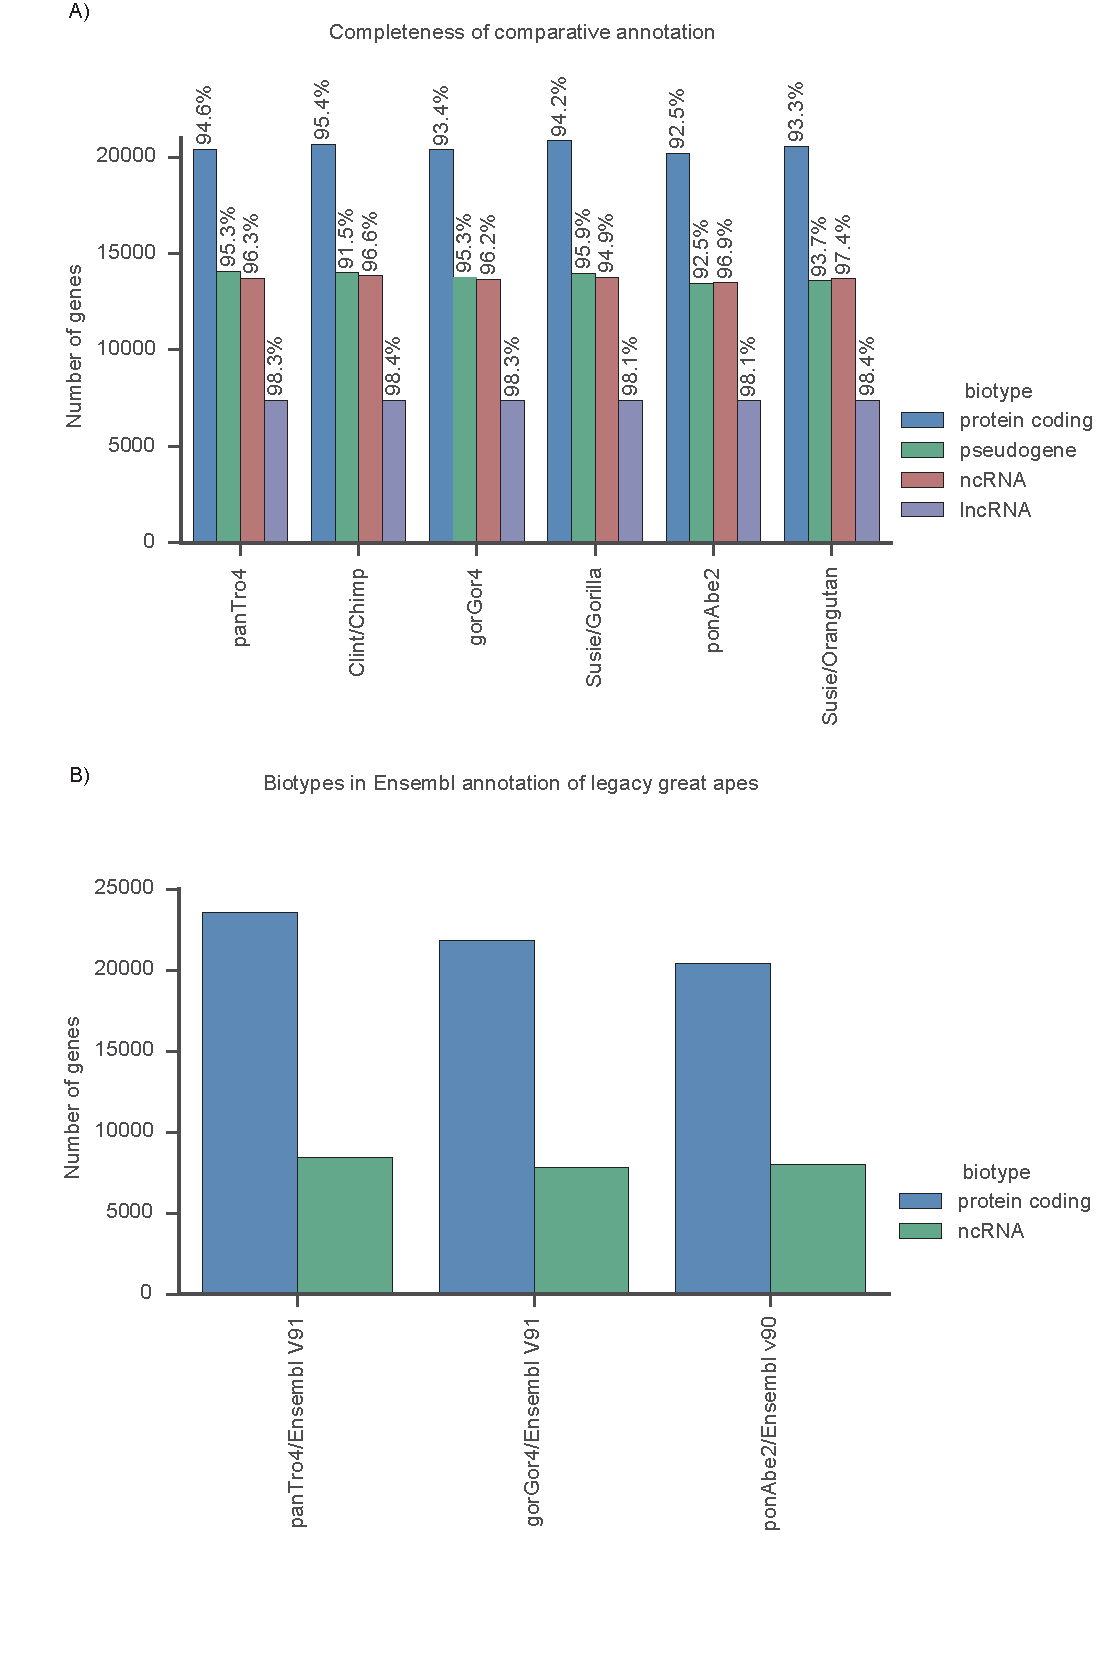
\includegraphics[scale=0.6]{Supplemental_Figure_S2.pdf}
\caption{Primate completeness and biotypes}
A) Percent of genes in simplified biotypes identified in both generations of great ape assemblies. The numbers above the bars are the percent of GENCODE V27 genes identified broken down by simplified biotypes. The number of genes identified in the PacBio assemblies increased slightly for all of the great apes. B) The biotypes of the Ensembl annotations for the older great apes. Compared to the 19,836 protein-coding genes in GENCODE V27, these annotation sets have 23,534, 21,795 and 20,424 protein-coding genes for chimpanzee, gorilla and orangutan respectively, suggesting misclassified noncoding loci. We found 940 loci in chimp, 1,728 loci in gorilla and 1,270 loci in orangutan, which are labeled as protein coding in Ensembl but are labeled other biotypes in the CAT annotation. Not only does CAT make tracking orthology relationships easier, but it also provides much higher correlation with real data, greatly improving cross-species RNA-seq analysis.
\label{supp_fig:primate_completeness}
\end{figure}

\begin{figure}
\centering
\includegraphics[width=\textwidth,height=\textheight,keepaspectratio]{Supplemental_Figure_S3.pdf}
\caption{Primate Coding Indels}
The rate of transcripts with coding indels seen in the consensus gene sets for the SMRT primate assemblies are shown with Quiver and Pilon correction (left), and subsequent Freebayes  \citep{garrison2012haplotype}-based correction (right). Freebayes correction was not performed on GSMRT5 (gorilla). Coding indels are measured by pairwise translated BLAT alignments of a transcript to its ortholog in human. SMRT assemblies show a systematic overrepresentation of coding deletions. After Freebayes correction, the rate of insertions to deletions is roughly equal and lower than the rate of multiple of 3 indels, which is the expected result due to purifying selection.
\label{supp_fig:primate_indels}
\end{figure}

\begin{figure}
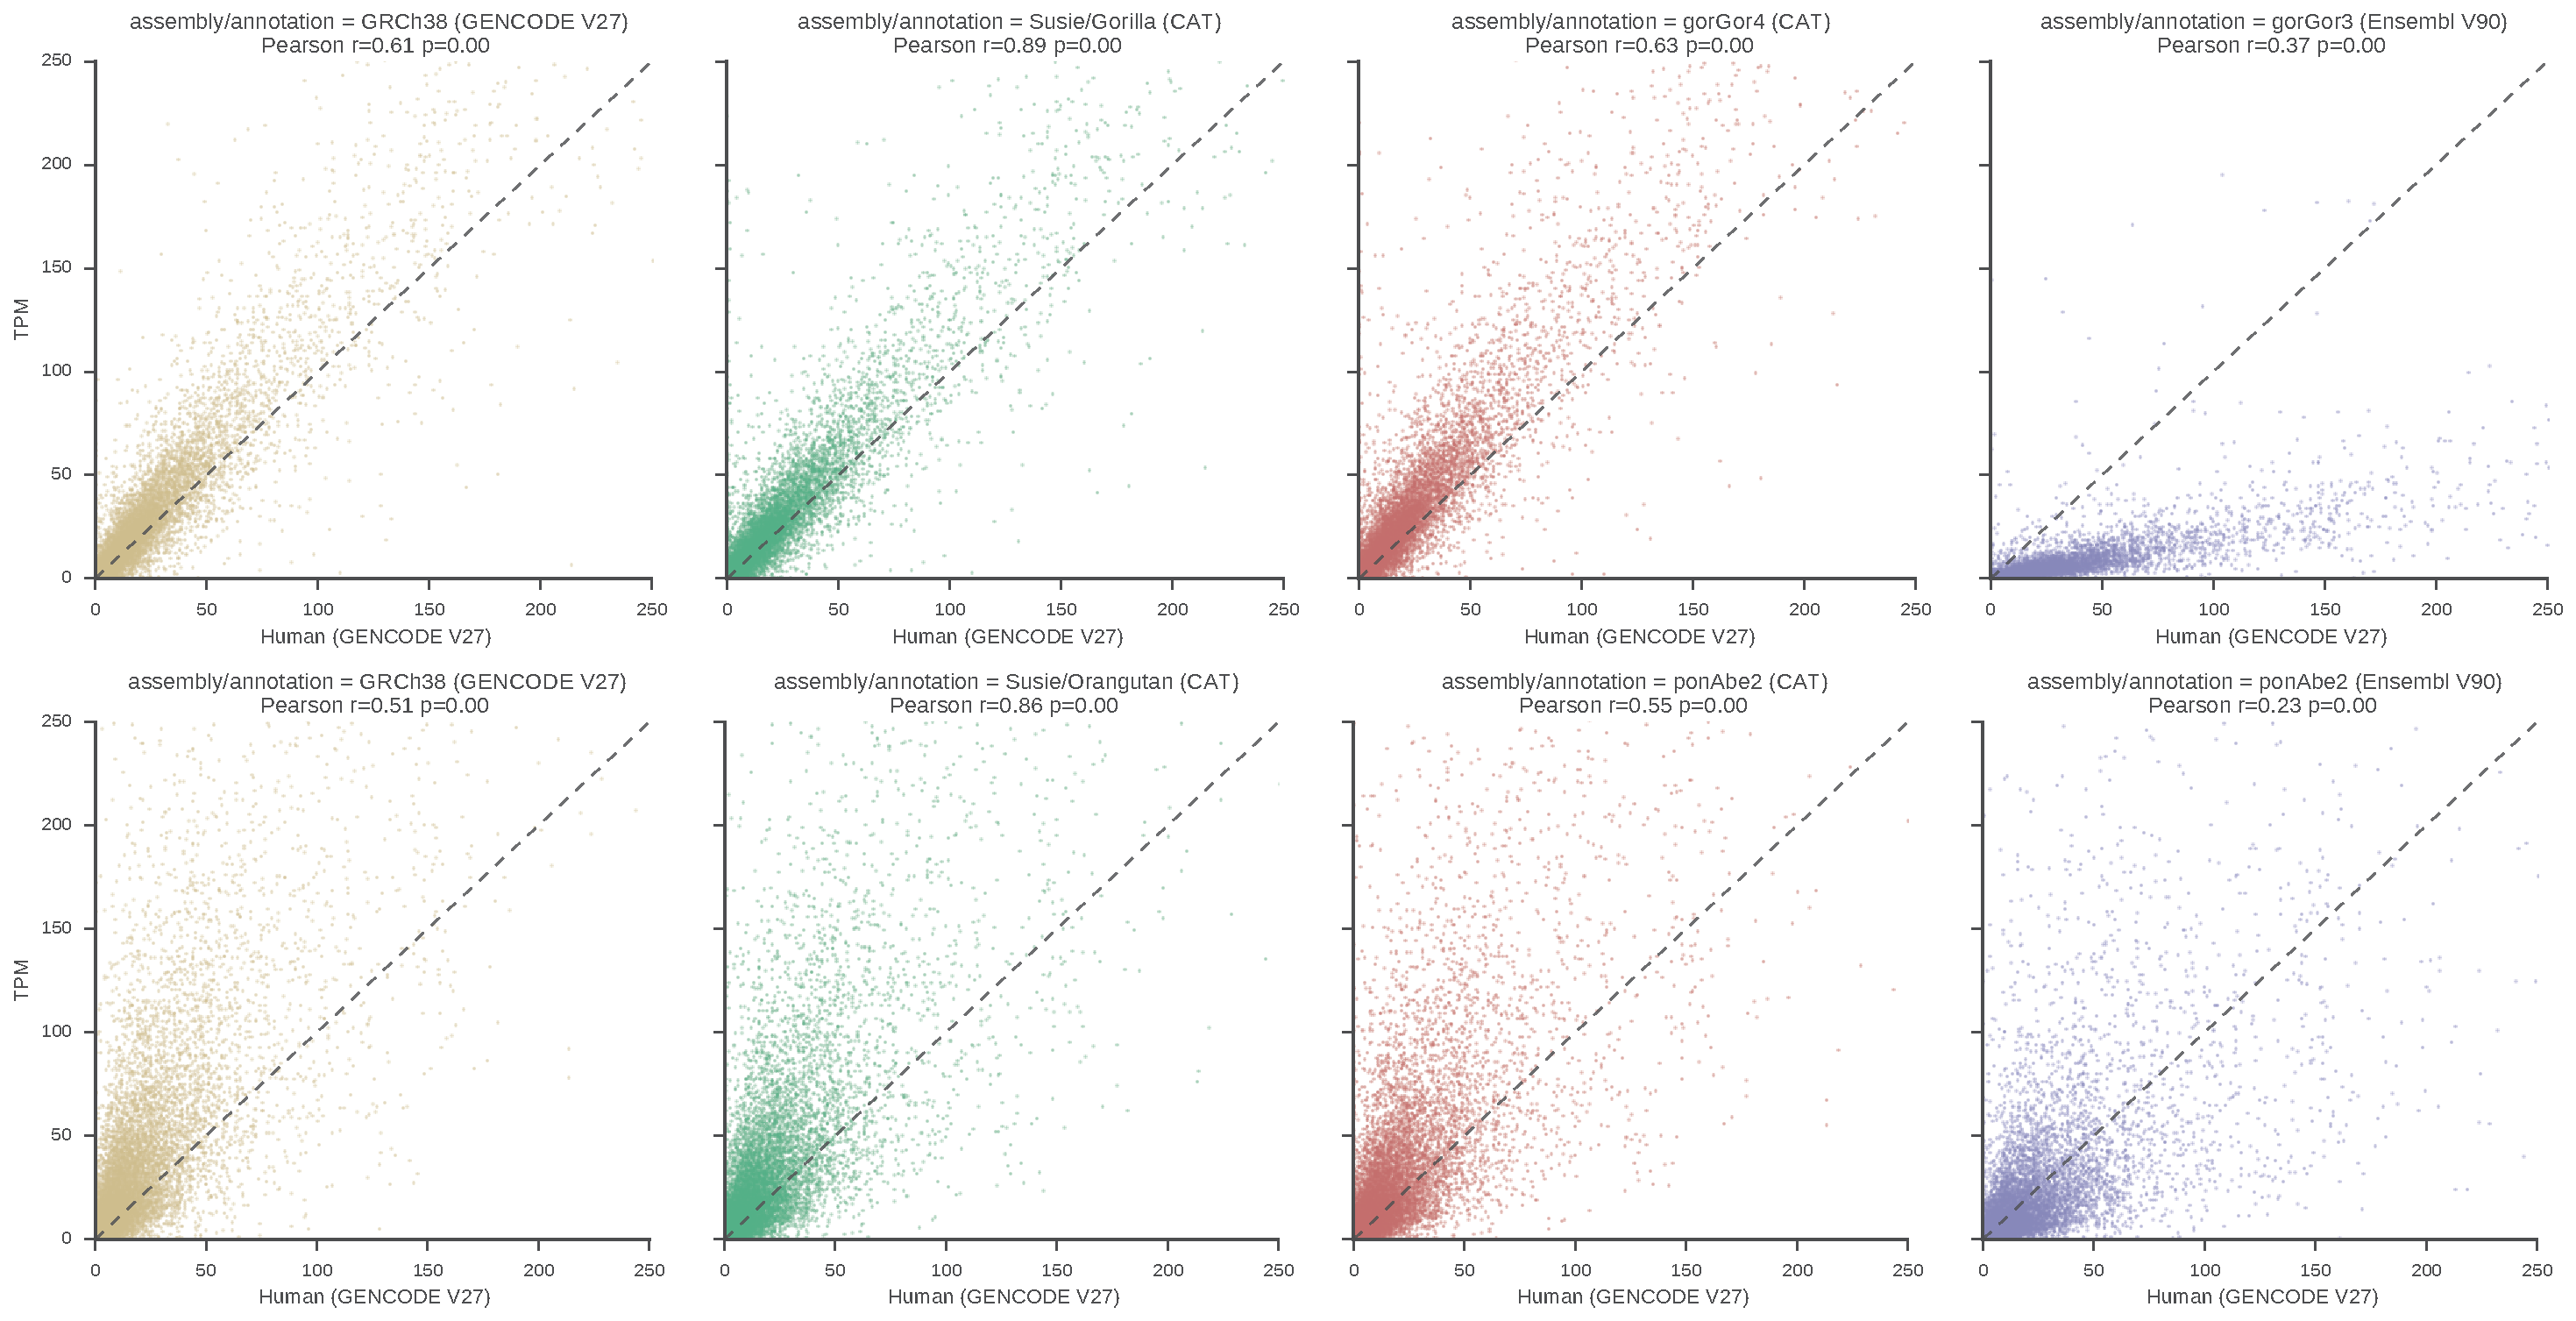
\includegraphics[width=0.8\paperwidth,keepaspectratio]{Supplemental_Figure_S4.pdf}
\caption{Cross-species RNA-seq expression estimates}

Gorilla and orangutan iPSC RNA-seq are compared to human iPSC RNA-seq using a variety of annotation and assembly combinations. All comparisons were performed with Kallisto. Cross-species comparison was used by tracking gene common names, and only protein-coding genes were considered. Because the pre-release of Ensembl V91 provided to us lacked common names, we used V90. Ensembl V90 annotation is on gorGor3, so that genome was used. The x-axes in all plots are the TPM of human iPSC data mapped to GENCODE V27. The y-axes in all plots are the TPM of species-specific iPSC RNA-seq mapped to the assembly/annotation pair in the title. In all cases, using the newest version of the assemblies with CAT provides the highest correlation.
\label{supp_fig:primate_expression}
\end{figure}

\begin{figure}

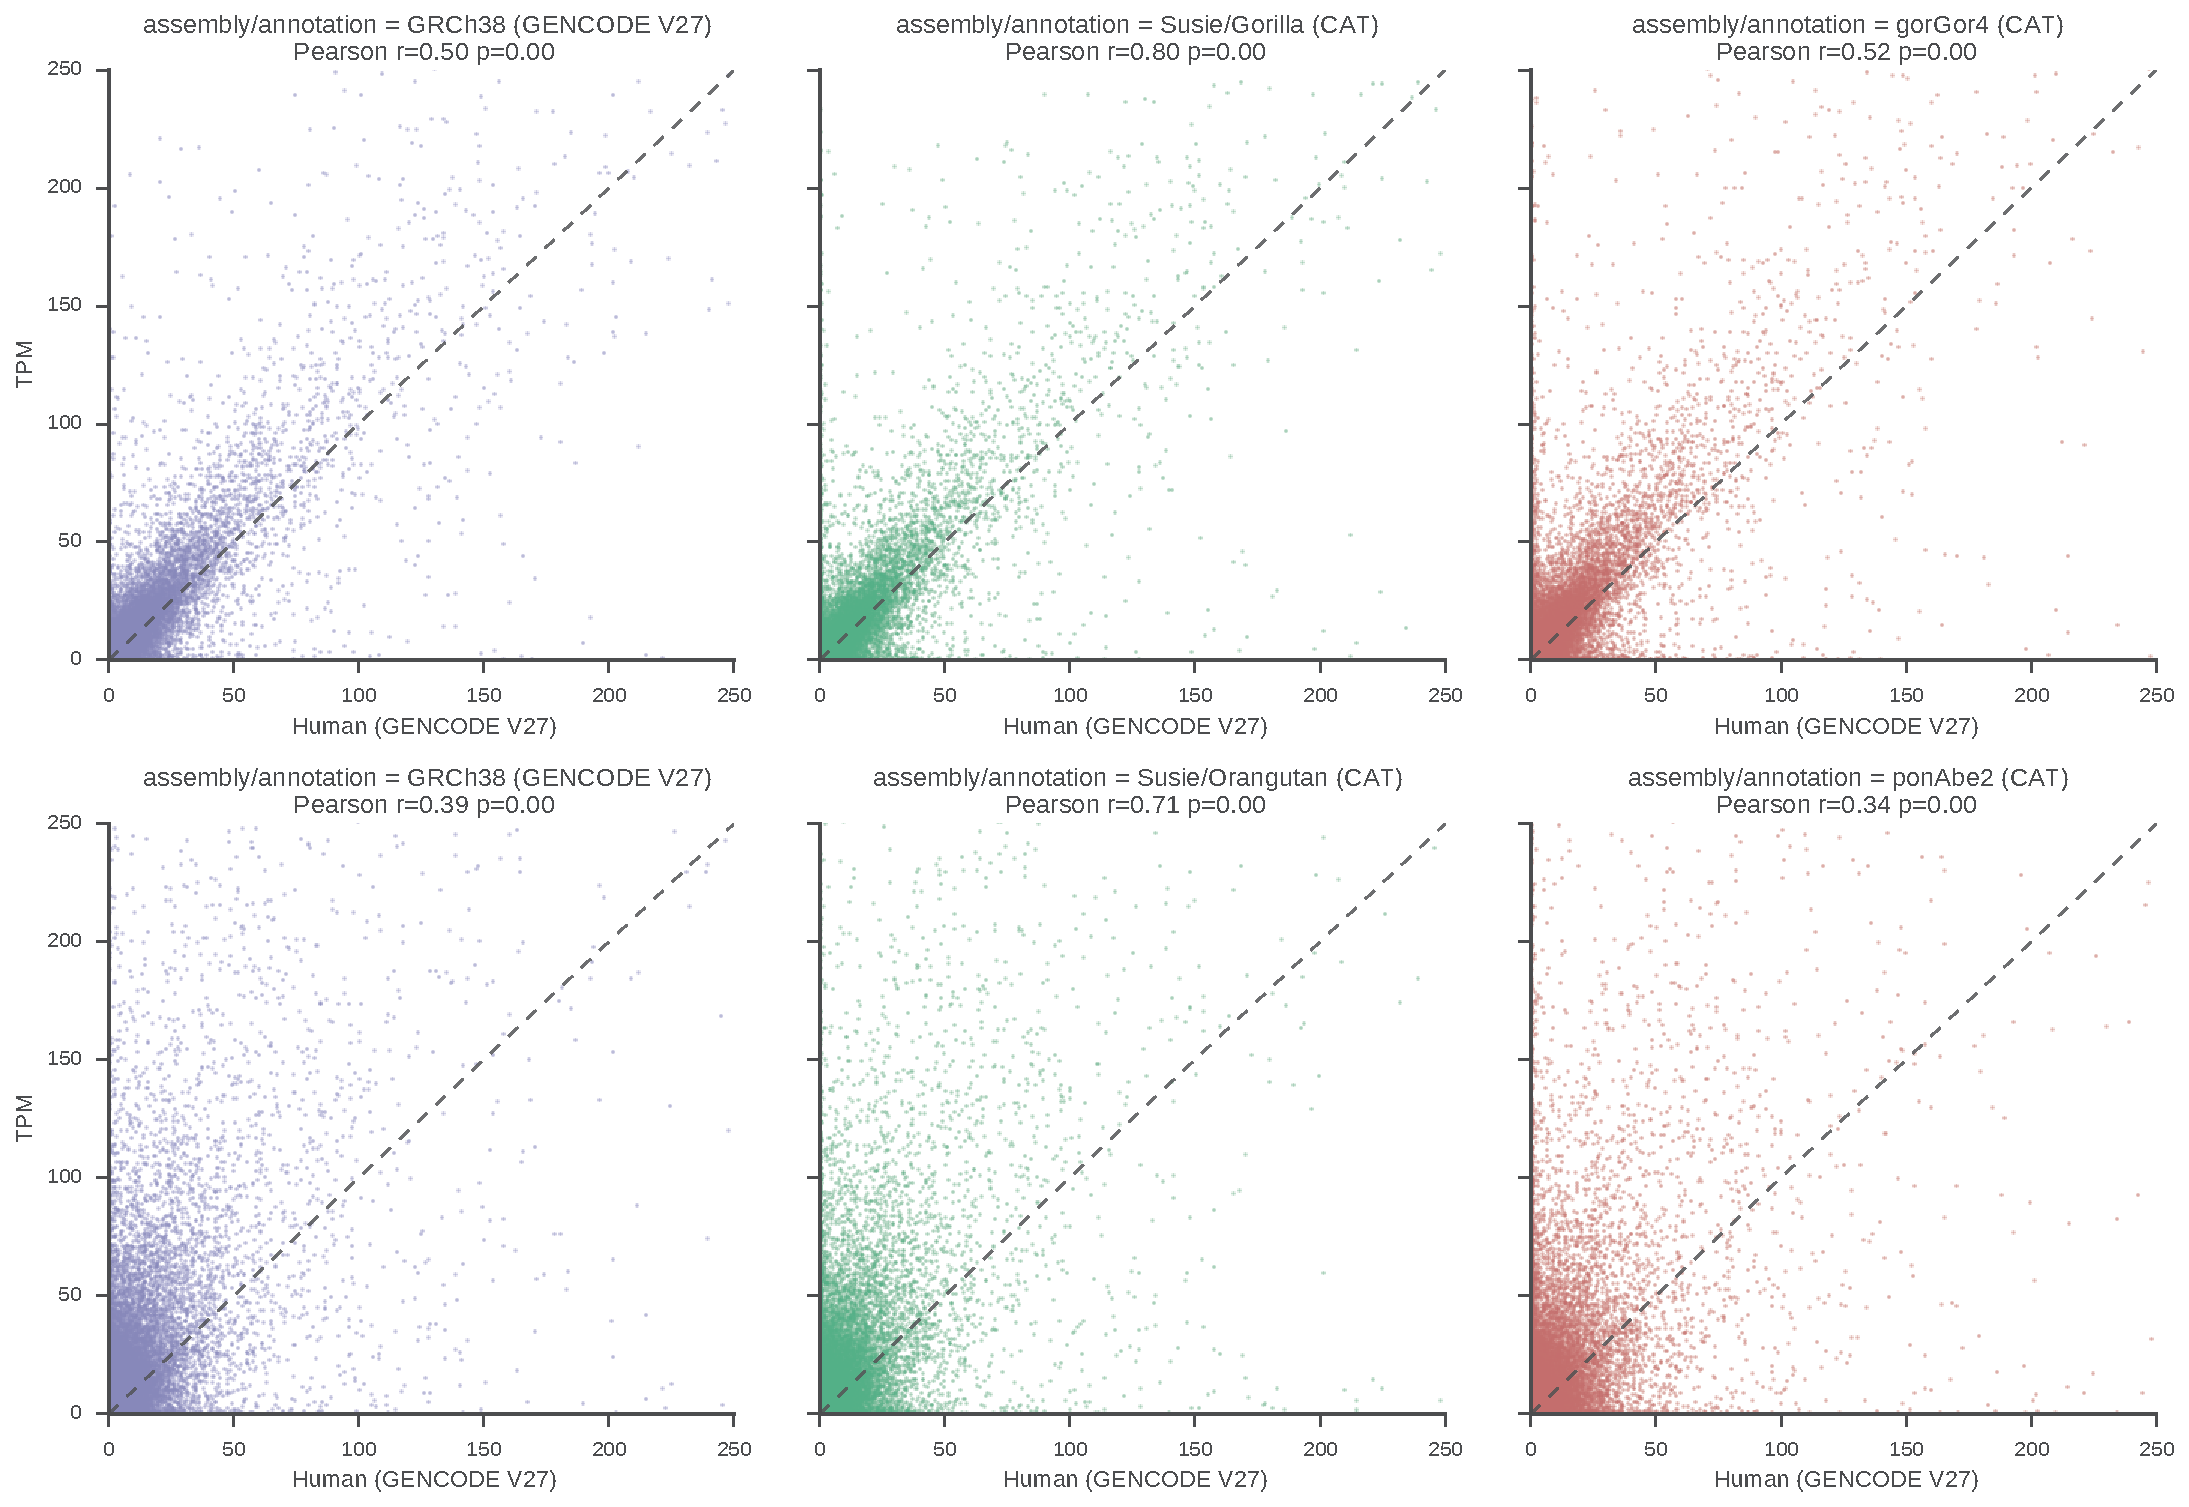
\includegraphics[width=0.8\paperwidth,keepaspectratio]{Supplemental_Figure_S5.pdf}

\caption{Cross-species RNA-seq isoform expression estimates}
The same analysis as in Figure \ref{fig:primate}D and Supplemental Figure \ref{supp_fig:primate_expression} was performed on the isoform level. For this analysis Ensembl was not included because we lacked a mapping of isoform IDs between the Ensembl annotation set and GENCODE. Only protein-coding isoforms were considered. The highest correlation is seem in CAT annotation of SMRT genomes, although correlation falls off considerably as phylogenetic distance increases from chimpanzee to orangutan.

\label{supp_fig:primate_transcript_expression}
\end{figure}

\begin{figure}
\centering
\includegraphics[width=\textwidth,height=\textheight,keepaspectratio]{Supplemental_Figure_S6.pdf}
\caption{Primate Split Genes}
\label{supp_fig:primate_split_genes}
Split gene analysis looks for transcript projections after paralog resolution that map to multiple contigs. This provides a metric for assembly contiguity. Despite the PacBio assemblies not being in chromosome-sized pieces, fewer split genes are detected, suggesting that most contig breaks are not in genic regions.
\end{figure}

\begin{figure}
\centering
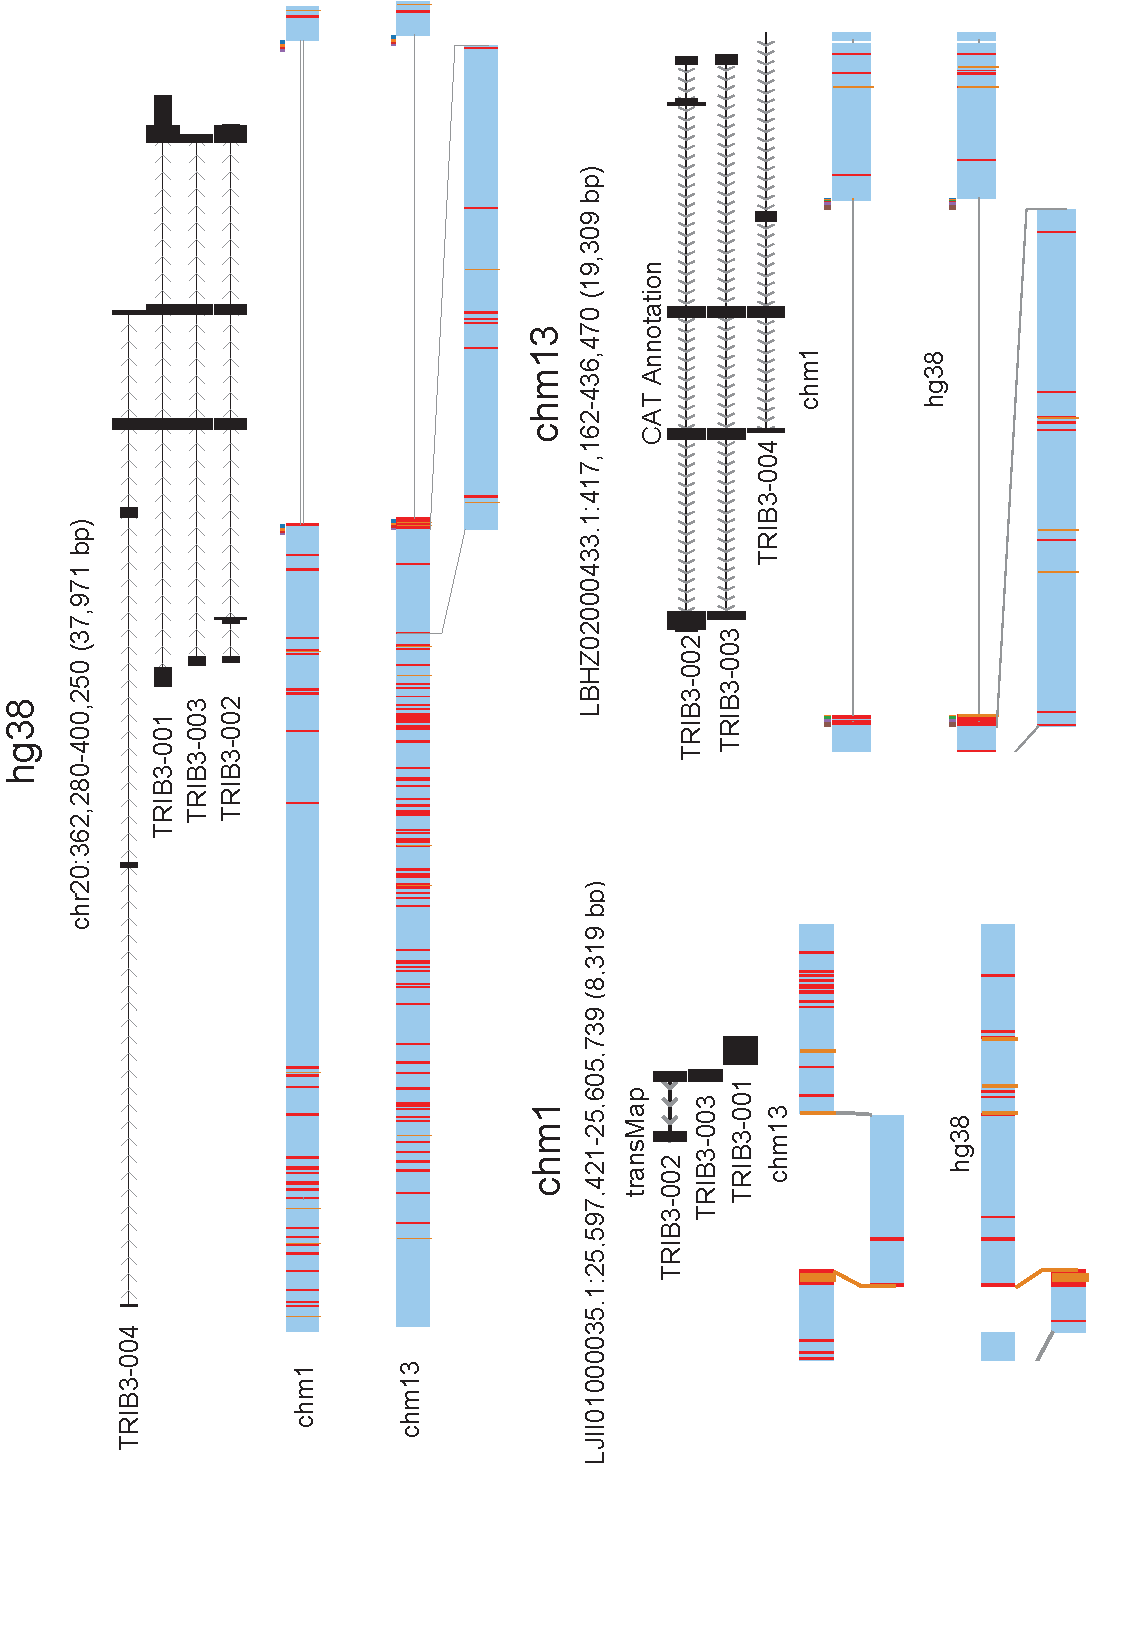
\includegraphics[width=0.8\textwidth,height=0.7\textheight,keepaspectratio]{Supplemental_Figure_S7.pdf}
\caption{\textit{TRIB3} example}
The CHM1 structural variant in figure 4 is shown here from all perspectives. In CHM1, the short transMaps for the few remaining exons are filtered out and do not end up in the annotation set. In contrast, CAT annotated 3/4 of the isoforms in CHM13. This figure shows the power of the UCSC assembly hub for evaluating structural variants by being able to view the alignment from any species present.
\label{supp_fig:trib3}
\end{figure}

\begin{figure}
\centering
\includegraphics[]{Supplemental_Figure_S8.pdf}
\caption{Rat completeness}
The number of genes comparatively identified in the rn6 assembly from mm10 GENCODE VM11, broken down by simplified biotypes. The percentages on top are the percent of the total genes in each simplified biotype present in VM11. While a large portion of protein-coding genes are identified, much fewer lncRNAs and other noncoding biotypes are identified.
\label{supp_fig:rat_completeness}
\end{figure}

\begin{figure}
\centering
\makebox[\textwidth]{\includegraphics[width=0.8\paperwidth]{Supplemental_Figure_S9.pdf}}
\caption{Rat Locus Venn Diagram}
Gene loci were compared between CAT, Ensembl V90, MAKER and RefSeq on rat rn6. Loci were clustered using the Kent tool clusterGenes, which requires exonic overlap on the same strand. Only 15,179 loci are shared between all sets.
\label{supp_fig:rat_locus_venn}
\end{figure}

\begin{figure}
\centering
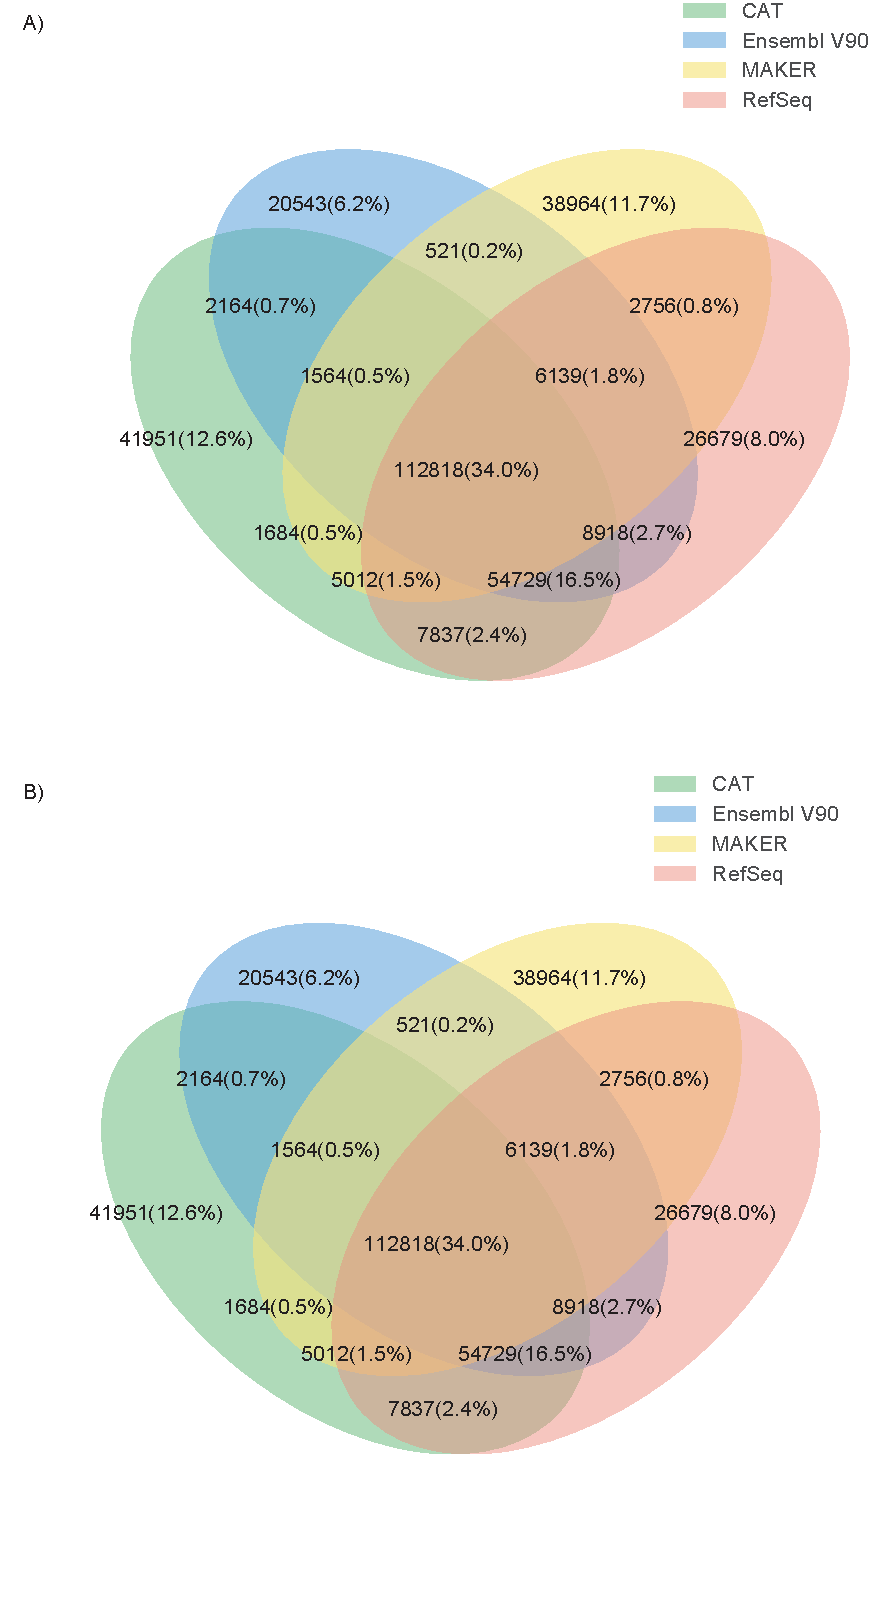
\includegraphics[width=0.5\paperwidth]{Supplemental_Figure_S10.pdf}
\caption{Rat Exon/Intron Support Venn Diagram}
CDS Intron (left) and CDS exon (right) interval exact matches were compared between CAT, Ensembl V90, MAKER and RefSeq on rat rn6. MAKER had the highest proportion of unsupported exons and introns, followed by CAT. Only 37.0\% and 34.0\% of introns and exons respectively are present in all four annotation sets.
\label{supp_fig:rat_exon_intron}
\end{figure}

\begin{figure}
\centering
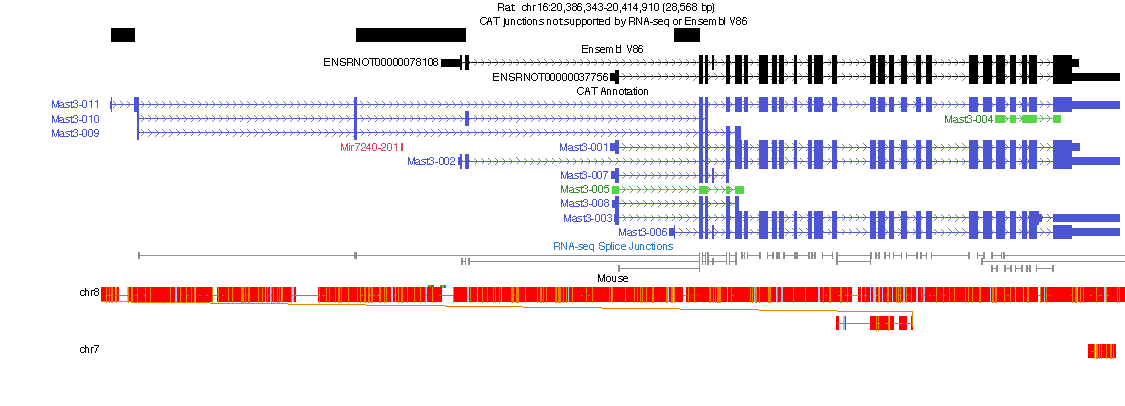
\includegraphics[width=\textwidth,height=\textheight,keepaspectratio,angle=90]{Supplemental_Figure_S11.pdf}
\caption{Unsupported junctions example}
The rat gene Mast3 has two annotated isoforms in Ensembl supported by RNA-seq. CAT annotation added 9 new isoforms, two of which had unsupported junctions. These new annotations reveal an upstream transcription initiation site supported by RNA-seq. 
\label{supp_fig:unsupported_junctions}
\end{figure}

\begin{table}
\centering
\begin{tabular}{|l|l|}
 \hline
Genome & Number of BUSCO genes missing \\ \hline
\textit{Mus pahari}      & 38 \\ \hline
Rat (rn6)      & 99 \\ \hline
Rhesus (rheMac3)   & 138 \\ \hline
Chimpanzee (panTro4) & 90 \\ \hline
Human (hg19)     & 26 \\ \hline
Gorilla (gorGor3)  & 184 \\ \hline
Orangutan (ponAbe2) & 133 \\ \hline
Cat (felCat8)    & 95 \\ \hline
Elephant (loxAfr3)  & 114 \\ \hline
Rabbit (oryCun2)   & 147 \\ \hline
Dog (canFam3)    & 90 \\ \hline
Sheep (oviAri3)   & 162 \\ \hline
Cow (bosTau8)    & 93 \\ \hline
\end{tabular}
\caption{BUSCO genes missing in 13 mammal annotation}
BUSCO  \citep{simao2015busco} was used to quantify the number of core key genes missing in the CAT annotation of 13 mammalian genomes. For this analysis, the mammalian odb\_9 set of 4,104 genes was used. BUSCO genes represent core housekeeping genes present at single copy across long evolutionary distance. On average, 108 BUSCO genes (2.63\%) are missing in each genome. Only three BUSCO genes (EOG090A0GHJ, EOG090A05ND, and EOG090A04MN) were missing in all 13 genomes.
\label{supp_table:busco}
\end{table}

\begin{center}
\small
\captionof{table}{SRA RNA-seq accessions}
\label{supp_table:rnaseq_sra_table}
\begin{longtable}{|p{0.15\textwidth}|p{0.65\textwidth}|p{0.2\textwidth}|} \hline
Species  & SRA Accessions & Tissues \\ \hline
Rat    & SRR1041777, SRR1768421, SRR1768443, SRR1768444, SRR299123, SRR636875, SRR636876, SRR636877, SRR636925, SRR636926, SRR636927, SRR636970, SRR636971, SRR636972                                                                                                                                          & Mixed, testis, liver, kidney, brain                                          \\ \hline
Orangutan & SRR306792, SRR2176206, SRR2176207                                                                                                                                                                                                       & Brain, testis                                                     \\ \hline
Gorilla  & SRR832925, SRR3053573, SRR306809, SRR306803, SRR306804, SRR306801, SRR306807, SRR306810, SRR306805, SRR306806, SRR306802, SRR306800, SRR306808                                                                                                                                                 & Brain, 20 tissue pool                                                 \\ \hline
Chimp   & SRR2040584, SRR2040585, SRR2040586, SRR2040587, SRR2040588, SRR2040589, SRR2040590, SRR2040591, SRR3711187, SRR3711188, SRR873622, SRR873623, SRR873624, SRR873625                                                                                                                                       & brain, heart, liver, testis, 8 week old iPSC derived neurons, undifferentiated iPSC                  \\ \hline
Rhesus  & SRR306784, SRR306786, SRR306785, SRR2040593, SRR306783, SRR306787, SRR306780, SRR306778, SRR306790, SRR2040595, SRR2040594, SRR2040592, SRR306788, SRR306782, SRR306789, SRR306777, SRR306779, SRR306781                                                                                                                    &  Kidney, liver, heart, brain, testis                                                          \\ \hline
Human   & ERR579132, ERR579133, ERR579134, ERR579135, ERR579136, ERR579137, ERR579138, ERR579139, ERR579140, ERR579141, ERR579142, ERR579143, ERR579144, ERR579145, ERR579146, ERR579147, ERR579148, ERR579149, ERR579150, ERR579151, ERR579152, ERR579153, ERR579154, ERR579155                                                                                     & Ovary, tonsil, fallopian tube, placenta, endometrium, rectum, skeletal muscle, liver, fat, colon, smooth muscle, lung \\ \hline
Sheep   & SRR1653601, SRR1561187, SRR1561150, SRR1265856, SRR1536790, SRR1561171, SRR1265854, SRR1561367, SRR1561365, SRR1653570, SRR1653598, SRR1653597, SRR1266019, SRR1265849, SRR1653600, SRR1656805, SRR1561366, SRR1653594, SRR1561196, SRR1265855, SRR1653596, SRR1536788, SRR1266022, SRR1561156, SRR1266018, SRR1561195, SRR1536770, SRR1266020                                                 &   Liver, brain, blood                                                          \\ \hline
Cow    & SRR2960011, SRR2960020, SRR2960008, SRR2960010, SRR2960012, SRR2960016, SRR2960006, SRR2960015, SRR2960025, SRR2960003, SRR2960022, SRR2960029, SRR2960030, SRR2960017, SRR2960032, SRR2960005, SRR2960027, SRR2960007, SRR2960036, SRR2960026, SRR2960035, SRR2960004, SRR2960002, SRR2960034, SRR2960013, SRR2960001, SRR2960021, SRR2960019, SRR2960009, SRR2960024, SRR2960014, SRR2960031, SRR2960033, SRR2960023, SRR2960028, SRR2960018 &  Liver, udder                                                          \\ \hline
Elephant & SRR1041765, SRR975189, SRR975188, SRR3222430                                                                                                                                                                                                  &    Fibroblast                                                        \\ \hline
Rabbit  & SRR636919, SRR636872, SRR636964, SRR636871, SRR636920, SRR636965                                                                                                                                                                                        &     Liver, kidney, brain                                                       \\ \hline
Cat    & SRR3200450, SRR3200448, SRR3200449, SRR3200453                                                                                                                                                                                                 &   Fetus, lung, liver                            \\ \hline              
\end{longtable}
Publicly available RNA-seq obtained via SRA for annotations performed in this paper. 
\end{center}